% !TeX program = xelatex
\documentclass[a4paper,10pt]{article}

% ============================================================================
% សន្លឹកកិច្ចការសិស្សបំពេញចន្លោះ ស-ខ្មៅ និងប្លង់ក្ដារខៀន/ចម្លើយគ្រូ (គ្មាន LCD / គ្មានកន្ត្រៃ)
% មេរៀនទី២ (៥.)៖ តួចែករួមធំបំផុត (PGCD ឬ GCD) — ត្រូវគ្នា ១០០% នឹង LS_Plan_DIV25.tex
% ============================================================================
\usepackage[a4paper, left=1.0cm, right=1.0cm, top=0.75cm, bottom=1.00cm, footskip=0.52cm]{geometry}
\usepackage{amsmath}
\usepackage{unicode-math}
\usepackage{fontspec}
\usepackage{array, colortbl}
\usepackage[table]{xcolor}
\usepackage{enumitem}
\usepackage{pifont}
\usepackage{fancyhdr}
\usepackage{lastpage}
\usepackage{tikz}
\usepackage[most]{tcolorbox}
\usetikzlibrary{calc, arrows.meta, decorations.pathreplacing, positioning, babel}

\makeatletter
\let\@expl@@@mark@update@singlecol@structures@@\relax
\makeatother

\providecommand{\NGSFindFonts}{%
  \IfFileExists{C:/Windows/Fonts/cambria.ttc}{%
    \def\NGSSysPath{C:/Windows/Fonts/}%
    \def\NGSUserPath{C:/Users/KIT/AppData/Local/Microsoft/Windows/Fonts/}%
  }{%
    \IfFileExists{./fonts/KhmerOSsiemreap.ttf}{\def\NGSSysPath{./fonts/}\def\NGSUserPath{./fonts/}}{%
    \IfFileExists{../fonts/KhmerOSsiemreap.ttf}{\def\NGSSysPath{../fonts/}\def\NGSUserPath{../fonts/}}{%
    \IfFileExists{../../fonts/KhmerOSsiemreap.ttf}{\def\NGSSysPath{../../fonts/}\def\NGSUserPath{../../fonts/}}{%
    \IfFileExists{../../../fonts/KhmerOSsiemreap.ttf}{\def\NGSSysPath{../../../fonts/}\def\NGSUserPath{../../../fonts/}}{%
    \IfFileExists{../../../../fonts/KhmerOSsiemreap.ttf}{\def\NGSSysPath{../../../../fonts/}\def\NGSUserPath{../../../../fonts/}}{%
    \IfFileExists{../../../../../fonts/KhmerOSsiemreap.ttf}{\def\NGSSysPath{../../../../../fonts/}\def\NGSUserPath{../../../../../fonts/}}{%
    \IfFileExists{../../../../../../fonts/KhmerOSsiemreap.ttf}{\def\NGSSysPath{../../../../../../fonts/}\def\NGSUserPath{../../../../../../fonts/}}{%
      \def\NGSSysPath{../../../../../../../fonts/}\def\NGSUserPath{../../../../../../../fonts/}%
    }}}}}}}%
  }%
}
\NGSFindFonts

\setmathfont[Path={\NGSSysPath}, FontIndex=1, Scale=1.02]{cambria.ttc}
\defaultfontfeatures{Ligatures=TeX}

\setmainfont[
  Path={\NGSUserPath}, Extension=.ttf, Script=Khmer,
  BoldFont={KhmerOSsiemreap}, BoldFeatures={FakeBold=1.8},
  ItalicFont={KhmerOSsiemreap}, ItalicFeatures={FakeSlant=0.25},
  BoldItalicFont={KhmerOSsiemreap}, BoldItalicFeatures={FakeBold=1.8, FakeSlant=0.25}
]{KhmerOSsiemreap}

\newfontfamily\muol[Path={\NGSUserPath}, Extension=.ttf, Script=Khmer]{KhmerOSmuollight}
\newfontfamily\TimesEn[Path={\NGSSysPath}, Extension=.ttf, BoldFont={timesbd}, ItalicFont={timesi}, BoldItalicFont={timesbi}]{times}
\newfontfamily\CalibriFont[Path={\NGSSysPath}, Extension=.ttf]{calibri}

\XeTeXlinebreaklocale "km"
\XeTeXlinebreakskip = 0pt plus 1pt minus 0.1pt

\definecolor{panelgray}{gray}{0.94}
\definecolor{headgray}{gray}{0.85}

\pagestyle{fancy}
\fancyhf{}
\renewcommand{\headrulewidth}{0pt}
\fancyfoot[L]{\fontsize{7.4pt}{9.5pt}\selectfont អនុវិទ្យាល័យព្រះក្រសាំង \en{|} គ្រូ៖ ហុក ប៊ុនថែន \en{|} មេរៀនទី២ (៥.) តួចែករួមធំបំផុត (\en{PGCD}) \en{|} ថ្ងៃអង្គារ ទី១៧ ខែវិច្ឆិកា ឆ្នាំ២០២៦}
\fancyfoot[R]{\fontsize{7.8pt}{10pt}\selectfont ទំព័រ \en{\thepage\ / \pageref{LastPage}}}

\setlength{\parindent}{0pt}
\setlength{\parskip}{0pt}
\setlength{\tabcolsep}{4pt}
\newcolumntype{L}[1]{>{\raggedright\arraybackslash}p{#1}}
\newcolumntype{C}[1]{>{\centering\arraybackslash}p{#1}}

\newcommand{\en}[1]{{\TimesEn #1}}
\newcommand{\enbf}[1]{{\TimesEn\bfseries #1}}
\newcommand{\unit}[1]{\,\text{\en{#1}}}
\newcommand{\cnum}[1]{\mbox{\fontsize{10pt}{12pt}\selectfont\ding{\numexpr181+#1\relax}}}
\newcommand{\chkbox}{\tikz[baseline=-0.15ex]\draw[black, line width=0.85pt, fill=white] (0,0) rectangle (0.24cm,0.24cm);}
\newcommand{\ansbox}[1][1.75cm]{\,\tikz[baseline=-0.65ex]\draw[black, line width=0.65pt, fill=white] (0,0) rectangle (#1, 0.42cm);\,}
\newcommand{\dotline}[1][2.2cm]{\makebox[#1]{\dotfill}}

\newcommand{\pagebanner}[2]{%
  \begin{tcolorbox}[
    enhanced, sharp corners, colback=headgray, colframe=black,
    boxrule=1.05pt, boxsep=1pt, top=2.5pt, bottom=2.5pt, left=6pt, right=6pt,
    after skip=3.5pt
  ]
    {\muol\fontsize{9.0pt}{13.2pt}\selectfont #1}\hfill{\fontsize{8.0pt}{11.2pt}\selectfont\textbf{#2}}
  \end{tcolorbox}%
}

\newcommand{\secstrip}[2]{%
  \vspace{3pt}%
  \begin{tcolorbox}[
    enhanced, sharp corners, colback=panelgray, colframe=black,
    boxrule=0.8pt, boxsep=0.8pt, top=2pt, bottom=2pt, left=5pt, right=5pt,
    after skip=3pt
  ]
    {\muol\fontsize{8.5pt}{12.2pt}\selectfont #1}\hfill{\fontsize{7.8pt}{10.8pt}\selectfont\textit{#2}}
  \end{tcolorbox}%
}

\begin{document}
\fontsize{9.5pt}{14.5pt}\selectfont

% ============================================================================
% ទំព័រទី ១៖ សន្លឹកកិច្ចការសិស្ស (ផ្នែកមុខ៖ E1 -> E2 -> E3)
% ============================================================================
\pagebanner{សន្លឹកកិច្ចការសិស្ស \enbf{(}៥\enbf{.} តួចែករួមធំបំផុត \enbf{PGCD} ឬ \enbf{GCD)} \enbf{--} ផ្នែកមុខ}{ថ្នាក់ទី៧ \en{|} សៀវភៅគោល ទំ.២១--២២}

\begin{tcolorbox}[
  enhanced, sharp corners, colback=white, colframe=black,
  boxrule=0.8pt, boxsep=1.5pt, top=3.5pt, bottom=3.5pt, left=5pt, right=5pt,
  after skip=4pt
]
  \fontsize{9.0pt}{13.0pt}\selectfont
  \textbf{ឈ្មោះសិស្ស៖} \dotline[4.3cm] \quad
  \textbf{សមាជិកក្រុម៖} \dotline[4.3cm] \quad
  \textbf{ថ្នាក់ទី៖} ៧\dotline[0.9cm] \quad
  \textbf{ក្រុមទី៖} \dotline[1.0cm]
\end{tcolorbox}

% --- E1 Engage ---
\secstrip{ផ្នែកទី ១ \enbf{(E1 - Engage)} ៖ បេសកកម្មអន្ទាក់ពាក្យ «ធំបំផុត» ក្នុង $\operatorname{PGCD}(12, 18)$}{រយៈពេល ៣ នាទី (គូស \ding{51} ក្នុង \chkbox)}

\begin{tcolorbox}[
  enhanced, sharp corners, colback=white, colframe=black,
  boxrule=0.8pt, boxsep=2pt, top=4pt, bottom=4pt, left=6pt, right=6pt
]
  គេដឹងថា $12 = 2^2 \times 3$ និង $18 = 2 \times 3^2$ ។ គេចង់រក\textbf{តួចែករួមធំបំផុត} $\operatorname{PGCD}(12, 18)$៖\\[2.5pt]
  $\bullet$ \chkbox\ \textbf{សិស្ស ក៖} «ព្រោះរកតួចែករួម\textbf{ធំបំផុត} ត្រូវយកនិទស្សន្តធំជាងគេ គឺ $2^2 \times 3^2 = 36$!»\\[2pt]
  $\bullet$ \chkbox\ \textbf{សិស្ស ខ៖} «$12$ ចែកមិនដាច់នឹង $36$ ទេ! ត្រូវយកកត្តារួមមាននិទស្សន្ត\textbf{តូចជាងគេ} គឺ $2 \times 3 = 6$ ទើបចែកដាច់ទាំងពីរ!»
\end{tcolorbox}

\vfill

% --- E2 Explore ---
\secstrip{ផ្នែកទី ២ \enbf{(E2 - Explore)} ៖ តារាងតម្រឹមជួរឈរកត្តាបឋមរួម (សៀវភៅគោល ទំ.២១)}{រយៈពេល ១១ នាទី}

\textbf{សកម្មភាព ១ (\en{E2-A} — ៥.៥ នាទី)៖ រក $\operatorname{PGCD}(30, 36)$ តាមវិធីទាំងពីរ (ឧទាហរណ៍ 1 ទំ.២១)}

\begin{tcolorbox}[
  enhanced, sharp corners, colback=white, colframe=black,
  boxrule=0.8pt, boxsep=2.5pt, top=4pt, bottom=4pt, left=6pt, right=6pt
]
  \begin{minipage}[t]{0.48\textwidth}
    \textbf{១) វិធីទី 1៖ រាយតួចែក}\\[2.5pt]
    $\bullet$ តួចែកនៃ $30$: $1, 2, 3,$ \dotline[0.6cm], \dotline[0.6cm], $10, 15, 30$\\[2.5pt]
    $\bullet$ តួចែកនៃ $36$: $1, 2, 3, 4,$ \dotline[0.6cm], $9, 12, 18, 36$\\[2.5pt]
    $\bullet$ តួចែករួម៖ $1, 2, 3,$ \dotline[0.7cm] $\implies \operatorname{PGCD} =$ \ansbox[1.1cm]
  \end{minipage}\hfill
  \vrule width 0.6pt\hfill
  \begin{minipage}[t]{0.48\textwidth}
    \textbf{២) វិធីទី 2៖ តម្រឹមជួរឈរកត្តាបឋម (គូសប្រអប់កត្តារួម)}\\[2.5pt]
    \hspace*{0.4cm}$30 = \;\;2\;\; \times \;\;3\;\; \times 5$\\[2pt]
    \hspace*{0.4cm}$36 = \;\;2^2\; \times \;\;3^2$\\[2.5pt]
    កត្តារួម (និទស្សន្តតូច)៖ $\operatorname{PGCD}(30, 36) =$ \dotline[0.7cm] $\times$ \dotline[0.7cm] $=$ \ansbox[1.1cm]
  \end{minipage}
\end{tcolorbox}

\vspace{4pt}
\textbf{សកម្មភាព ២ (\en{E2-B} — ៥.៥ នាទី)៖ ចំនួនបីតួ និងចំនួនបឋមរវាងគ្នា (ឧទាហរណ៍ 2 និង 3 ទំ.២១)}

\begin{tcolorbox}[
  enhanced, sharp corners, colback=white, colframe=black,
  boxrule=0.8pt, boxsep=2.5pt, top=4.5pt, bottom=4.5pt, left=6pt, right=6pt
]
  \begin{minipage}[t]{0.52\textwidth}
    \textbf{១) ឧទាហរណ៍ 2៖ រក $\operatorname{PGCD}(60, 180, 210)$}\\[2pt]
    \hspace*{0.2cm}$60\phantom{0} = 2^2 \times 3\phantom{^2} \times 5$\\
    \hspace*{0.2cm}$180 = 2^2 \times 3^2 \times 5$\\
    \hspace*{0.2cm}$210 = 2\phantom{^2} \times 3\phantom{^2} \times 5 \times 7$\\[2.5pt]
    $\operatorname{PGCD}(60, 180, 210) =$ \dotline[0.7cm] $\times$ \dotline[0.7cm] $\times$ \dotline[0.7cm] $=$ \ansbox[1.3cm]
  \end{minipage}\hfill
  \vrule width 0.6pt\hfill
  \begin{minipage}[t]{0.44\textwidth}
    \textbf{២) ឧទាហរណ៍ 3៖ ចំនួនបឋមរវាងគ្នា}\\[2pt]
    $\bullet$ $\operatorname{PGCD}(11, 13) =$ \ansbox[1.1cm]\\[2.5pt]
    $\bullet$ $8 = 2^3$ និង $15 = 3 \times 5$ (គ្មានកត្តាបឋមរួម)\\[2pt]
    $\implies \operatorname{PGCD}(8, 15) =$ \ansbox[1.1cm] (បឋមរវាងគ្នា!)
  \end{minipage}
\end{tcolorbox}

\vfill

% --- E3 Explain ---
\secstrip{ផ្នែកទី ៣ \enbf{(E3 - Explain)} ៖ វិធានទូទៅ ចំនួនបឋមរវាងគ្នា និងធនាគារហេតុផល \enbf{B\&W}}{រយៈពេល ៦ នាទី}

\begin{tcolorbox}[
  enhanced, sharp corners, colback=white, colframe=black,
  boxrule=0.85pt, boxsep=2.5pt, top=4pt, bottom=4pt, left=6pt, right=6pt
]
  $\bullet$ \textbf{ជាទូទៅ (ទំ.២១)៖} ដើម្បីរក $\operatorname{PGCD}$ នៃពីរឬច្រើនចំនួន គេបំបែកចំនួននីមួយៗជាផលគុណកត្តាបឋម រួចគុណ\textbf{កត្តា\dotline[1.6cm]ទាំងអស់ ដែលមាននិទស្សន្ត\dotline[2.4cm]} ។\\[2.5pt]
  $\bullet$ \textbf{សម្គាល់ (ទំ.២១)៖} ពីរចំនួន\textbf{បឋមរវាងគ្នា} កាលណា $\operatorname{PGCD}$ របស់វាស្មើនឹង \dotline[1.0cm] ។\\[3pt]
  \tikz\draw[black, dashed, line width=0.5pt] (0,0) -- (18.4cm,0);\\[3pt]
  \fontsize{8.7pt}{12.8pt}\selectfont
  \textbf{ធនាគារហេតុផល (\en{Warrant Bank})៖} \quad
  \cnum{1} $\operatorname{PGCD}(a,b)$ ត្រូវចែកដាច់ទាំង $a$ និង $b$ ($\le \min(a,b)$) \quad
  \cnum{2} ជ្រើស\textbf{តែកត្តាបឋមរួម} (ផាត់ចោលកត្តាមិនរួម)\\
  \cnum{3} ជ្រើស\textbf{និទស្សន្តតូចជាងគេ}នៃកត្តារួម រួចគុណគ្នា \qquad
  \cnum{4} បើគ្មានកត្តាបឋមរួម នោះ $\operatorname{PGCD} = 1$ (បឋមរវាងគ្នា)
\end{tcolorbox}

% ============================================================================
% ទំព័រទី ២៖ សន្លឹកកិច្ចការសិស្ស (ផ្នែកខាងខ្នង៖ E4 -> E5 -> កិច្ចការផ្ទះ)
% ============================================================================
\clearpage
\pagebanner{សន្លឹកកិច្ចការសិស្ស \enbf{(}៥\enbf{.} តួចែករួមធំបំផុត \enbf{PGCD} ឬ \enbf{GCD)} \enbf{--} ផ្នែកខាងខ្នង}{ថ្នាក់ទី៧ \en{|} សៀវភៅគោល ទំ.២១--២២ និង ទំ.២៤}

% --- E4 Elaborate ---
\secstrip{ផ្នែកទី ៤ \enbf{(E4 - Elaborate)} ៖ លំហាត់គំរូតាមសៀវភៅគោល ទំ.២១--២២ (ក្រាលឥដ្ឋការ៉ូការេ)}{រយៈពេល ១០ នាទី}

\begin{tcolorbox}[
  enhanced, sharp corners, colback=white, colframe=black,
  boxrule=0.8pt, boxsep=2.5pt, top=4.5pt, bottom=4.5pt, left=6pt, right=6pt
]
  \textbf{ប្រធាន (ទំ.២១)៖} គេចង់ក្រាលឥដ្ឋការ៉ូរាងការេមានទំហំប៉ុនៗគ្នាឱ្យពេញលើផ្ទៃបន្ទប់ទឹករាងចតុកោណកែង ដែលមានទទឹង $90\unit{cm}$ និងបណ្ដោយ $126\unit{cm}$ ។ បើគេចង់ក្រាលឥដ្ឋការ៉ូដែលមានផ្ទៃធំបំផុត តើត្រូវប្រើឥដ្ឋការ៉ូប៉ុន្មាន? មានជ្រុងប្រវែងប៉ុន្មាន?\\[4pt]
  \begin{minipage}[t]{0.60\textwidth}
    $\bullet$ \textbf{១) បំបែកកត្តាបឋម៖}\\[2pt]
    \hspace*{0.3cm}$90\phantom{0} = 2 \times$ \dotline[1.0cm] $\times 5$ \qquad និង \qquad $126 = 2 \times$ \dotline[1.0cm] $\times 7$\\[3pt]
    $\bullet$ \textbf{២) ប្រវែងជ្រុងការ៉ូធំបំផុត៖} $\operatorname{PGCD}(90, 126) =$ \dotline[1.6cm] $=$ \ansbox[2.0cm] (\cnum{2}, \cnum{3})\\[3pt]
    $\bullet$ \textbf{៣) ចំនួនការ៉ូត្រូវប្រើ៖} $(90 \div 18) \times (126 \div 18) =$ \dotline[0.8cm] $\times$ \dotline[0.8cm] $=$ \ansbox[2.0cm] សន្លឹក
  \end{minipage}\hfill
  \begin{minipage}[t]{0.37\textwidth}
    \vspace{2pt}
    \centering
    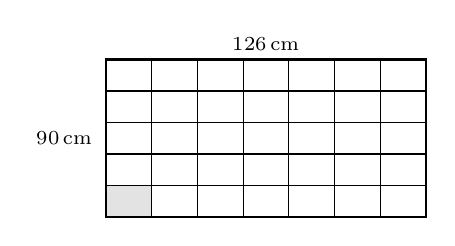
\begin{tikzpicture}[x=1cm, y=1cm, every node/.style={font=\fontsize{7.2pt}{9.2pt}\selectfont, text=black}]
      \fill[gray!22] (0,0) rectangle (0.58,0.40);
      \draw[black, line width=0.8pt] (0,0) rectangle (4.06,2.00);
      \foreach \i in {1,...,6} {\draw[black, line width=0.4pt] (\i*0.58,0) -- (\i*0.58,2.00);}
      \foreach \j in {1,...,4} {\draw[black, line width=0.4pt] (0,\j*0.40) -- (4.06,\j*0.40);}
      \node at (2.03,2.20) {$126\unit{cm}$};
      \node[anchor=east] at (-0.06,1.00) {$90\unit{cm}$};
    \end{tikzpicture}
  \end{minipage}\\[4pt]
  \tikz\draw[black, dashed, line width=0.5pt] (0,0) -- (18.4cm,0);\\[3pt]
  \fontsize{8.8pt}{12.8pt}\selectfont
  \textbf{ឆ្លុះបញ្ចាំង (\en{EIA Looking-Back})៖} ចំណោទដែលតម្រូវឱ្យ\textbf{កាត់បំបែក ឬចែកស្មើៗគ្នា}ជាចំណែកធំបំផុតដោយគ្មានសល់ គឺត្រូវប្រើ \dotline[2.0cm] ជានិច្ច!
\end{tcolorbox}

\vfill

% --- E5 Evaluate ---
\secstrip{ផ្នែកទី ៥ \enbf{(E5 - Evaluate)} ៖ ប្រតិបត្តិ (ទំ.២២) សំណួរវិនិច្ឆ័យ \enbf{A--D} និងសំបុត្រចេញ}{រយៈពេល ១០ នាទី}

\begin{tcolorbox}[
  enhanced, sharp corners, colback=white, colframe=black,
  boxrule=0.8pt, boxsep=2.5pt, top=4.5pt, bottom=4.5pt, left=6pt, right=6pt
]
  \textbf{១) ប្រតិបត្តិជាក្រុមតូច ៣ នាក់ (សៀវភៅគោល ទំ.២២)៖} គេចែកសៀវភៅ $24$ ក្បាល និងខ្មៅដៃ $36$ ដើមឱ្យសិស្សស្មើៗគ្នាដោយគ្មានឱ្យសល់សៀវភៅ ឬខ្មៅដៃ ។ តើគេអាចចែកឱ្យសិស្សបានច្រើនបំផុតប៉ុន្មាននាក់?\\[3pt]
  $\bullet$ បំបែក៖ $24 =$ \dotline[1.8cm] \quad និង \quad $36 =$ \dotline[1.8cm] $\implies \operatorname{PGCD}(24, 36) =$ \ansbox[2.2cm] នាក់ (\cnum{2}, \cnum{3})\\[3pt]
  $\bullet$ ក្នុងម្នាក់ៗទទួលបាន៖ សៀវភៅ $24 \div 12 =$ \dotline[0.9cm] ក្បាល \quad និង \quad ខ្មៅដៃ $36 \div 12 =$ \dotline[0.9cm] ដើម ។\\[3.5pt]
  \textbf{២) បិទបេសកកម្ម \en{E1}៖} សិស្ស \dotline[1.0cm] ត្រឹមត្រូវ! $\operatorname{PGCD}(12, 18) =$ \ansbox[1.5cm] ។
\end{tcolorbox}

\vspace{4pt}

\begin{tcolorbox}[
  enhanced, sharp corners, colback=white, colframe=black,
  boxrule=0.8pt, boxsep=2.5pt, top=4.5pt, bottom=4.5pt, left=6pt, right=6pt
]
  \textbf{៣) សំណួរវិនិច្ឆ័យ \en{A--D} (គេឱ្យ $A = 2^3 \times 3^2 \times 5$ និង $B = 2^2 \times 3^4 \times 7$ — តើ $\operatorname{PGCD}(A, B)$ ស្មើមួយណា?)៖}\\[3.5pt]
  \textbf{\en{A.}} $2^3 \times 3^4 \times 5 \times 7$ \qquad
  \textbf{\en{B.}} $2^2 \times 3^2 \times 5 \times 7$ \qquad
  \textbf{\en{C.}} $2^2 \times 3^2 = 36$ \qquad
  \textbf{\en{D.}} $2^3 \times 3^4 = 648$\\[4pt]
  \tikz\draw[black, dashed, line width=0.5pt] (0,0) -- (18.4cm,0);\\[3.5pt]
  \textbf{៤) សំបុត្រចេញ ៦០ វិនាទី៖} រកតួចែករួមធំបំផុតនៃ $45$ និង $75$៖ $45 =$ \dotline[1.5cm], $75 =$ \dotline[1.5cm] $\implies \operatorname{PGCD}(45, 75) =$ \ansbox[1.8cm] ។
\end{tcolorbox}

\vfill

% --- Homework ---
\begin{tcolorbox}[
  enhanced, sharp corners, colback=panelgray, colframe=black,
  boxrule=0.95pt, boxsep=2.5pt, top=4pt, bottom=4pt, left=6pt, right=6pt
]
  {\muol\fontsize{9.0pt}{13.0pt}\selectfont កិច្ចការផ្ទះ \enbf{(}សៀវភៅគោល ទំ.២៤ លេខ ៦, លេខ ៨ និង លេខ ១០\enbf{)}}\\[2.5pt]
  \fontsize{8.7pt}{12.6pt}\selectfont
  $\bullet$ \textbf{លេខ ៦៖} រក $\operatorname{PGCD}$ នៃ៖ ក. $9$ និង $15$;\; ខ. $10$ និង $108$;\; គ. $128$ និង $324$;\; ឃ. $192, 160$ និង $96$;\; ង. $48, 72$ និង $132$;\; ច. $36, 168, 144$ និង $252$ ។\\[2pt]
  $\bullet$ \textbf{លេខ ៨៖} រកចំនួន $x$ និង $y$ ($0 < x < y$) ដោយដឹងថា $\operatorname{PGCD}(x, y) = 12$ និង $x + y = 72$ ។\\[2pt]
  $\bullet$ \textbf{លេខ ១០៖} កញ្ញារត្នីចង់កាត់ក្រណាត់រាងចតុកោណកែងទទឹង $24\unit{cm}$ និងបណ្ដោយ $56\unit{cm}$ ធ្វើកូនកន្សែងដៃរាងការេធំបំផុតដោយមិនឱ្យសល់ក្រណាត់ ។ រកប្រវែងជ្រុងកូនកន្សែងដៃ ។
\end{tcolorbox}

% ============================================================================
% ទំព័រទី ៣៖ ទំព័រគ្រូបង្រៀន (គំរូប្លង់ក្ដារខៀន ៣ ផ្នែក + ចម្លើយផ្ទៀងផ្ទាត់រហ័ស)
% ============================================================================
\clearpage
\pagebanner{ទំព័រគ្រូបង្រៀន ៖ ប្លង់ក្ដារខៀន \enbf{(}គ្មាន \enbf{LCD)} និងចម្លើយផ្ទៀងផ្ទាត់រហ័ស}{៥. តួចែករួមធំបំផុត \en{PGCD} (\en{DIV25})}

\secstrip{១. គំរូប្លង់បែងចែកក្ដារខៀន ៣ ផ្នែក សម្រាប់ថ្នាក់រៀនគ្មាន \enbf{LCD}}{សម្រាប់គ្រូប្រើដីស/ហ្វឺត}

\begin{center}
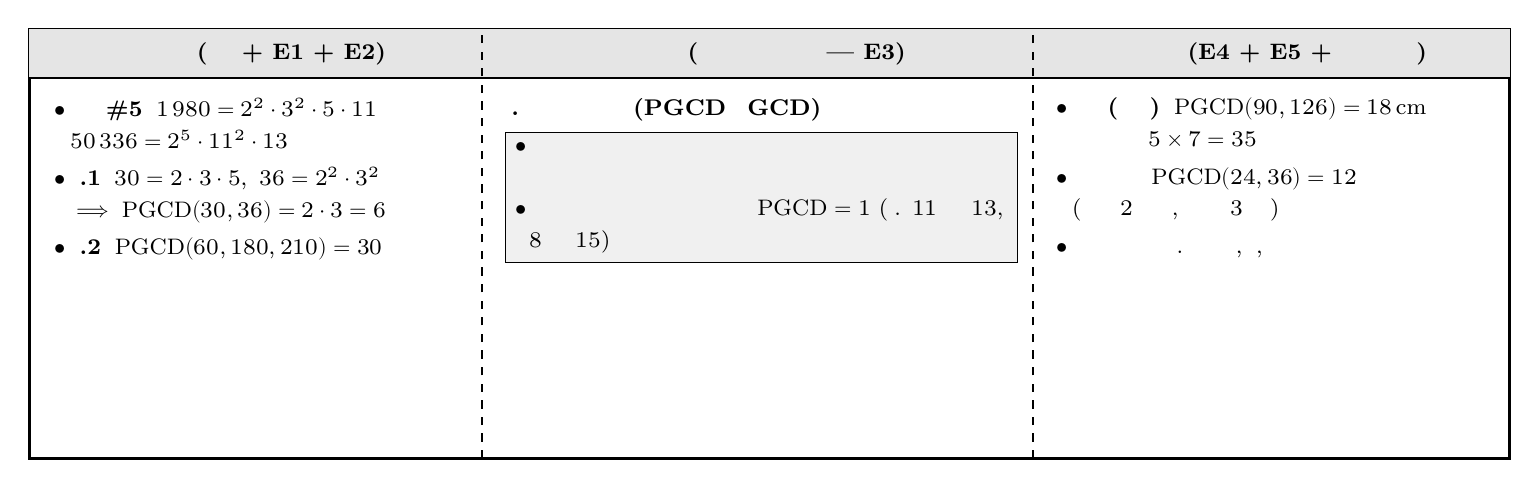
\begin{tikzpicture}[x=1cm, y=1cm, every node/.style={font=\fontsize{8.1pt}{11.5pt}\selectfont, text=black}]
  \draw[black, line width=1.1pt] (0,0) rectangle (18.8,5.45);
  \fill[gray!20] (0,4.83) rectangle (18.8,5.45);
  \draw[black, line width=0.7pt] (0,4.83) -- (18.8,4.83);
  \draw[black, dashed, line width=0.7pt] (5.75,0) -- (5.75,5.45);
  \draw[black, dashed, line width=0.7pt] (12.75,0) -- (12.75,5.45);

  \node at (2.875,5.14) {\textbf{ផ្នែកឆ្វេង (កំណែ + \en{E1} + \en{E2})}};
  \node at (9.25,5.14) {\textbf{ផ្នែកកណ្ដាល (ខ្លឹមសារគោលរក្សាទុក — \en{E3})}};
  \node at (15.775,5.14) {\textbf{ផ្នែកស្ដាំ (\en{E4} + \en{E5} + កិច្ចការផ្ទះ)}};

  % Left
  \node[anchor=north west, text width=5.30cm] at (0.20,4.70) {%
    $\bullet$ \textbf{កំណែ \#5៖} $1\,980 = 2^2\cdot 3^2\cdot 5\cdot 11$\\
    \hspace*{0.2cm}$50\,336 = 2^5\cdot 11^2\cdot 13$\\[2pt]
    $\bullet$ \textbf{ឧ.1៖} $30=2\cdot 3\cdot 5,\ 36=2^2\cdot 3^2$\\
    \hspace*{0.2cm}$\implies \operatorname{PGCD}(30,36) = 2\cdot 3 = 6$\\[2pt]
    $\bullet$ \textbf{ឧ.2៖} $\operatorname{PGCD}(60,180,210)=30$
  };

  % Center
  \node[anchor=north west, text width=6.65cm] at (5.92,4.70) {%
    {\muol\fontsize{8.2pt}{11.8pt}\selectfont ៥\enbf{.} តួចែករួមធំបំផុត \enbf{(PGCD} ឬ \enbf{GCD)}}\\[3pt]
    \tikz\node[draw=black, fill=gray!12, inner sep=3.5pt, text width=6.25cm]{%
      $\bullet$ \textbf{ជាទូទៅ៖} បំបែកចំនួននីមួយៗជាផលគុណកត្តាបឋម រួចគុណ\textbf{កត្តារួមទាំងអស់ដែលមាននិទស្សន្តតូចជាងគេ} ។\\
      $\bullet$ \textbf{សម្គាល់៖} ពីរចំនួន\textbf{បឋមរវាងគ្នា} កាលណា $\operatorname{PGCD} = 1$ (ឧ. $11$ និង $13$, ឬ $8$ និង $15$) ។
    };
  };

  % Right
  \node[anchor=north west, text width=5.65cm] at (12.92,4.70) {%
    $\bullet$ \textbf{គំរូ (ការ៉ូ)៖} $\operatorname{PGCD}(90,126) = 18\unit{cm}$\\
    \hspace*{0.2cm}ចំនួនការ៉ូ៖ $5\times 7 = 35$ សន្លឹក\\[2pt]
    $\bullet$ \textbf{ប្រតិបត្តិ៖} $\operatorname{PGCD}(24,36) = 12$ នាក់\\
    \hspace*{0.2cm}(សៀវភៅ $2$ ក្បាល, ខ្មៅដៃ $3$ ដើម)\\[2pt]
    $\bullet$ \textbf{កិច្ចការផ្ទះ៖} ទំ.២៤ លេខ ៦, ៨, ១០
  };
\end{tikzpicture}
\end{center}

\vfill
\secstrip{២. ចម្លើយផ្ទៀងផ្ទាត់រហ័សសម្រាប់សន្លឹកកិច្ចការសិស្ស \enbf{(}ទំព័រ ១ និង ទំព័រ ២\enbf{)}}{\en{Answer Key}}

\begin{tcolorbox}[
  enhanced, sharp corners, colback=white, colframe=black,
  boxrule=0.8pt, boxsep=2.5pt, top=4pt, bottom=4pt, left=6pt, right=6pt
]
  \fontsize{8.8pt}{12.9pt}\selectfont
  $\bullet$ \textbf{ផ្នែក \en{E1}៖} \textbf{សិស្ស ខ} ត្រឹមត្រូវ ($\operatorname{PGCD}(12,18)=6$) ។ \textbf{ផ្នែក \en{E2}៖} \en{E2-A}: $\operatorname{PGCD}(30,36)=\mathbf{6}$; \en{E2-B}: $\operatorname{PGCD}(60,180,210)=2\times 3\times 5=\mathbf{30}$, $\operatorname{PGCD}(11,13)=\mathbf{1}$, $\operatorname{PGCD}(8,15)=\mathbf{1}$ ។\\[2pt]
  $\bullet$ \textbf{ផ្នែក \en{E4}៖} $90=2\times 3^2\times 5$, $126=2\times 3^2\times 7 \implies \operatorname{PGCD}=\mathbf{18\unit{cm}}$; ចំនួនការ៉ូ $5\times 7 = \mathbf{35}$ សន្លឹក ។ \en{EIA}៖ $\operatorname{PGCD}$ ។\\[2pt]
  $\bullet$ \textbf{ផ្នែក \en{E5}៖} ១) $24=2^3\times 3,\ 36=2^2\times 3^2 \implies \mathbf{12}$ នាក់ ($2$ ក្បាល, $3$ ដើម) ។ ៣) \textbf{ជម្រើស \en{C}} ($36$) ។ ៤) សំបុត្រចេញ៖ $\operatorname{PGCD}(45,75)=\mathbf{15}$ ។
\end{tcolorbox}

\vfill
\secstrip{៣. ចម្លើយលម្អិតនៃកិច្ចការផ្ទះ \enbf{(}សៀវភៅគោល ទំ.២៤ លេខ ៦, លេខ ៨ និង លេខ ១០\enbf{)}}{សៀវភៅគោល ទំ.២៤}

\begin{tcolorbox}[
  enhanced, sharp corners, colback=white, colframe=black,
  boxrule=0.8pt, boxsep=2.5pt, top=4pt, bottom=4pt, left=6pt, right=6pt
]
  \fontsize{8.5pt}{12.5pt}\selectfont
  $\bullet$ \textbf{លេខ ៦៖} ក. $\operatorname{PGCD}(9,15)=\mathbf{3}$;\; ខ. $\operatorname{PGCD}(10,108)=\mathbf{2}$;\; គ. $128=2^7,\ 324=2^2\cdot 3^4 \implies \mathbf{4}$;\; ឃ. $192=2^6\cdot 3,\ 160=2^5\cdot 5,\ 96=2^5\cdot 3 \implies 2^5=\mathbf{32}$;\; ង. $48=2^4\cdot 3,\ 72=2^3\cdot 3^2,\ 132=2^2\cdot 3\cdot 11 \implies 2^2\cdot 3=\mathbf{12}$;\; ច. $36=2^2\cdot 3^2,\ 168=2^3\cdot 3\cdot 7,\ 144=2^4\cdot 3^2,\ 252=2^2\cdot 3^2\cdot 7 \implies 2^2\cdot 3=\mathbf{12}$ ។\\[2pt]
  $\bullet$ \textbf{លេខ ៨៖} តាង $x=12a,\ y=12b$ ដែល $\operatorname{PGCD}(a,b)=1$ និង $0<a<b$ ។ ដោយ $x+y=72 \implies 12(a+b)=72 \implies a+b=6$ ។ គូ $(a,b)$ ដែល $a<b$ និង $\operatorname{PGCD}(a,b)=1$ គឺ $(1, 5)$ ប៉ុណ្ណោះ (ព្រោះ $(2,4)$ មាន $\operatorname{PGCD}=2\ne 1$) $\implies \mathbf{x = 12,\ y = 60}$ ។\\[2pt]
  $\bullet$ \textbf{លេខ ១០៖} $24 = 2^3\times 3$ និង $56 = 2^3\times 7 \implies$ ជ្រុងកូនកន្សែងដៃការេធំបំផុតស្មើ $\operatorname{PGCD}(24, 56) = 2^3 = \mathbf{8\unit{cm}}$ (បាន $3\times 7 = 21$ កូនកន្សែង) ។
\end{tcolorbox}

\vfill
\secstrip{៤. ចំណុចប្រុងប្រយ័ត្នគរុកោសល្យសម្រាប់គ្រូ \enbf{(}អន្ទាក់ក្នុងលំហាត់ លេខ ៨\enbf{)}}{\en{Pedagogical Watchlist}}

\begin{tcolorbox}[
  enhanced, sharp corners, colback=panelgray, colframe=black,
  boxrule=0.85pt, boxsep=2.5pt, top=4pt, bottom=4pt, left=6pt, right=6pt
]
  \fontsize{8.5pt}{12.5pt}\selectfont
  $\bullet$ \textbf{អន្ទាក់គូ $(24, 48)$ ក្នុងលំហាត់លេខ ៨៖} សិស្សច្រើនជ្រើស $(a,b)=(2,4)$ បាន $x=24,\ y=48$ ដែលបូកឃើញ $72$ មែន ប៉ុន្តែ $\operatorname{PGCD}(24, 48) = 24 \ne 12$! ត្រូវរំលឹកសិស្សឱ្យផ្ទៀងលក្ខខណ្ឌបឋមរវាងគ្នា $\operatorname{PGCD}(a,b)=1$ ជានិច្ច ។
\end{tcolorbox}

\end{document}
